\documentclass[a4paper,12pt]{article}

\usepackage{amsmath}
\usepackage{graphicx}
\usepackage{tabularx}
\usepackage{xcolor}
\usepackage{listings}

\renewcommand*{\thesection}{\hspace{-5mm}}
\renewcommand*{\thesubsection}{(\alph{subsection})}

\setlength{\parindent}{0em}

\definecolor{Red}{RGB}{255, 0, 0}
\definecolor{Blue}{RGB}{0, 0, 255}

\begin{document}
	
	\title{Mixed-Effects Models, Spring 2022}
	\author{Mathieu Simon}
	\maketitle
	
	\setlength{\parskip}{1em}
	
	\section{Exercise 1}
	
	\subsection{}
		Steps reproduced until the plot\\
		\includegraphics[width=\linewidth]{Images/OatsPlot}
		
	\subsection{}
%		Data structure:\par
%		\includegraphics[width=0.6\linewidth]{Images/OatsModel}\\
		
%		Model:\\[0.5em]
		\begin{lstlisting}[language=R]
lme(yield~nitro, data=Oats, random=~1|Block/Variety)
		\end{lstlisting}
		
		$ \mathbf{y}_{ij} = \mathbf{X}_{ij}\boldsymbol\beta + \mathbf{Z}_{i,j}\mathbf{b}_i + \mathbf{Z}_{ij}\mathbf{b}_{ij} + \boldsymbol\epsilon_{ij}$\\
		
		Fixed effect:\\[0.5em]
		\begin{tabular}{m{5mm} c m{45mm} l}
			$\boldsymbol\beta$ &:& Nitrogen level & $p$ = 2  (intercept + slope)\\
		\end{tabular}\\
		
		Random effects:\\[0.5em]
		\begin{tabular}{m{5mm} c m{45mm} l}
			$\mathbf{b}_i$ &:& Block & $q_1$ = 1 (intercept)\\
			$\mathbf{b}_{ij}$ &:& Variety within block & $q_2$ = 1 (intercept)\\
		\end{tabular}\\
		
		Matrices:\\[0.5em]
		\begin{tabularx}{1\textwidth}{>{\centering\arraybackslash}X
									  >{\centering\arraybackslash}X
									  >{\centering\arraybackslash}X
									  >{\centering\arraybackslash}X
									  >{\centering\arraybackslash}X}
			$\mathbf{X}_{ij}$ & $\mathbf{Z}_{i,j}$ & $\mathbf{Z}_{ij}$ & $\boldsymbol\Psi_1$ & $\boldsymbol\Psi_2$
			\\[0.5em]
			$\begin{bmatrix}
				1 & 0.0 \\
				1 & 0.2 \\
				1 & 0.4 \\
				1 & 0.6 \\
			\end{bmatrix}$ & 
			$\begin{bmatrix}
				1 \\
				1 \\
				1 \\
				1 \\
			\end{bmatrix}$ & 
			$\begin{bmatrix}
				1 \\
				1 \\
				1 \\
				1 \\
			\end{bmatrix}$ & 
			$\begin{bmatrix}
				\sigma_1^2
			\end{bmatrix}$ & 
			$\begin{bmatrix}
				\sigma_2^2
			\end{bmatrix}$\\
		\end{tabularx}		
	
	\subsection{}
		Equivalent model specification:\\
		\begin{lstlisting}[language=R]
library(nlme)
lme(yield~nitro, data=Oats, random=list(Block=~1, Variety=~1))
		\end{lstlisting}
		Or
		\begin{lstlisting}[language=R]
library(lme4)
lmer(yield~nitro + (1|Block) + (1|Variety:Block), data=Oats)
		\end{lstlisting}
%		$\mathbf{y}_{i} = \mathbf{X}_{i}\boldsymbol\beta + \mathbf{Z}_{i}\tilde{\mathbf{b}}_i + \boldsymbol\epsilon_{ij}$\\
%		
%		With:\\[0.5em]
%		\begin{tabularx}{1\textwidth}{>{\centering\arraybackslash}X
%				>{\centering\arraybackslash}X
%				>{\centering\arraybackslash}X}
%			$\mathbf{X}_{i}$ & $\mathbf{Z}_{i}$ & $\tilde{\mathbf{b}}_{i}$
%			\\[0.5em]
%			$\begin{bmatrix}
%				\mathbf{X}_{i1} \\
%				\mathbf{X}_{i2} \\
%				\mathbf{X}_{i3} \\
%			\end{bmatrix}$ & 
%			$\begin{bmatrix}
%				\mathbf{Z}_{i,1} & \mathbf{Z}_{i1} & 0 & 0 \\
%				\mathbf{Z}_{i,2} & 0 & \mathbf{Z}_{i2} & 0 \\
%				\mathbf{Z}_{i,3} & 0 & 0 & \mathbf{Z}_{i2} \\
%			\end{bmatrix}$ & 
%			$\begin{bmatrix}
%				\mathbf{b}_{i} \\
%				\mathbf{b}_{i1} \\
%				\mathbf{b}_{i2} \\
%				\mathbf{b}_{i3} \\
%			\end{bmatrix}$\\
%		\end{tabularx}\\[0.5em]
%	
%		And:  $\tilde{\mathbf{b}}_{i} \sim N\left(\mathbf{0},\begin{bmatrix}
%			\boldsymbol{\Psi}_i & 0 & 0 & 0 \\
%			0 & \boldsymbol{\Psi}_2 & 0 & 0 \\
%			0 & 0 & \boldsymbol{\Psi}_2 & 0 \\
%			0 & 0 & 0 & \boldsymbol{\Psi}_2 \\
%		\end{bmatrix}\right)$
		
		\section{Exercise 2}
		$Var(\mathbf{y}_i) = \mathbf{Z}_{i}\boldsymbol{\Psi}\mathbf{Z}_{i}^T + \sigma^2\mathbf{I}_{n_i} =$\\[1em]
		$\begin{bmatrix}
			C_{11} & C_{12} & C_{13} & \quad C_{14} & C_{15} & C_{16} & \quad C_{17} & C_{18} & C_{19} \\
			C_{21} & C_{22} & C_{23} & \quad C_{24} & C_{25} & C_{26} & \quad C_{27} & C_{28} & C_{29} \\
			C_{31} & C_{32} & C_{33} & \quad C_{34} & C_{35} & C_{36} & \quad C_{37} & C_{38} & C_{39} \\[1em]
			C_{41} & C_{42} & C_{43} & \quad C_{44} & C_{45} & C_{46} & \quad C_{47} & C_{48} & C_{49} \\
			C_{51} & C_{52} & C_{53} & \quad C_{54} & C_{55} & C_{56} & \quad C_{57} & C_{58} & C_{59} \\
			C_{61} & C_{62} & C_{63} & \quad C_{64} & C_{65} & C_{66} & \quad C_{67} & C_{68} & C_{69} \\[1em]
			C_{71} & C_{72} & C_{73} & \quad C_{74} & C_{75} & C_{76} & \quad C_{77} & C_{78} & C_{79} \\
			C_{81} & C_{82} & C_{83} & \quad C_{84} & C_{85} & C_{86} & \quad C_{87} & C_{88} & C_{89} \\
			C_{91} & C_{92} & C_{93} & \quad C_{94} & C_{95} & C_{96} & \quad C_{97} & C_{98} & C_{99} \\
		\end{bmatrix}$
		
		\subsection{}
		$\begin{bmatrix}
			C_{1} & C_{2} & C_{2} & \quad C_{2} & C_{2} & C_{2} & \quad C_{2} & C_{2} & C_{2} \\
			C_{2} & C_{1} & C_{2} & \quad C_{2} & C_{2} & C_{2} & \quad C_{2} & C_{2} & C_{2} \\
			C_{2} & C_{2} & C_{1} & \quad C_{2} & C_{2} & C_{2} & \quad C_{2} & C_{2} & C_{2} \\[1em]
			C_{2} & C_{2} & C_{2} & \quad C_{1} & C_{2} & C_{2} & \quad C_{2} & C_{2} & C_{2} \\
			C_{2} & C_{2} & C_{2} & \quad C_{2} & C_{1} & C_{2} & \quad C_{2} & C_{2} & C_{2} \\
			C_{2} & C_{2} & C_{2} & \quad C_{2} & C_{2} & C_{1} & \quad C_{2} & C_{2} & C_{2} \\[1em]
			C_{2} & C_{2} & C_{2} & \quad C_{2} & C_{2} & C_{2} & \quad C_{1} & C_{2} & C_{2} \\
			C_{2} & C_{2} & C_{2} & \quad C_{2} & C_{2} & C_{2} & \quad C_{2} & C_{1} & C_{2} \\
			C_{2} & C_{2} & C_{2} & \quad C_{2} & C_{2} & C_{2} & \quad C_{2} & C_{2} & C_{1} \\
		\end{bmatrix}$
		
	
		\subsection{}
		$\begin{bmatrix}
			C_{1} & C_{2} & C_{2} & \quad C_{3} & C_{3} & C_{3} & \quad C_{3} & C_{3} & C_{3} \\
			C_{2} & C_{1} & C_{2} & \quad C_{3} & C_{3} & C_{3} & \quad C_{3} & C_{3} & C_{3} \\
			C_{2} & C_{2} & C_{1} & \quad C_{3} & C_{3} & C_{3} & \quad C_{3} & C_{3} & C_{3} \\[1em]
			C_{3} & C_{3} & C_{3} & \quad C_{1} & C_{2} & C_{2} & \quad C_{3} & C_{3} & C_{3} \\
			C_{3} & C_{3} & C_{3} & \quad C_{2} & C_{1} & C_{2} & \quad C_{3} & C_{3} & C_{3} \\
			C_{3} & C_{3} & C_{3} & \quad C_{2} & C_{2} & C_{1} & \quad C_{3} & C_{3} & C_{3} \\[1em]
			C_{3} & C_{3} & C_{3} & \quad C_{3} & C_{3} & C_{3} & \quad C_{1} & C_{2} & C_{2} \\
			C_{3} & C_{3} & C_{3} & \quad C_{3} & C_{3} & C_{3} & \quad C_{2} & C_{1} & C_{2} \\
			C_{3} & C_{3} & C_{3} & \quad C_{3} & C_{3} & C_{3} & \quad C_{2} & C_{2} & C_{1} \\
		\end{bmatrix}$
	
		\subsection{}
		$\begin{bmatrix}
			C_{1} & C_{4} & C_{4} & \quad C_{7} & C_{7} & C_{7} & \quad C_{8} & C_{8} & C_{8} \\
			C_{4} & C_{1} & C_{4} & \quad C_{7} & C_{7} & C_{7} & \quad C_{8} & C_{8} & C_{8} \\
			C_{4} & C_{4} & C_{1} & \quad C_{7} & C_{7} & C_{7} & \quad C_{8} & C_{8} & C_{8} \\[1em]
			C_{7} & C_{7} & C_{7} & \quad C_{2} & C_{5} & C_{5} & \quad C_{9} & C_{9} & C_{9} \\
			C_{7} & C_{7} & C_{7} & \quad C_{5} & C_{2} & C_{5} & \quad C_{9} & C_{9} & C_{9} \\
			C_{7} & C_{7} & C_{7} & \quad C_{5} & C_{5} & C_{2} & \quad C_{9} & C_{9} & C_{9} \\[1em]
			C_{8} & C_{8} & C_{8} & \quad C_{9} & C_{9} & C_{9} & \quad C_{3} & C_{6} & C_{6} \\
			C_{8} & C_{8} & C_{8} & \quad C_{9} & C_{9} & C_{9} & \quad C_{6} & C_{3} & C_{6} \\
			C_{8} & C_{8} & C_{8} & \quad C_{9} & C_{9} & C_{9} & \quad C_{6} & C_{6} & C_{3} \\
		\end{bmatrix}$

		
		
		
	
	
\end{document}
